% !TEX root = main.tex

\section{Теоретическая часть}

\subsection{Аппроксимация неизвестной зависимости}

Предположим, что в нашем распоряжении имеются результаты $n$ наблюдений:
\begin{equation}
\begin{cases}
    y_1 = \Phi(x_1) + \varepsilon_1 \\
    \qquad\cdots                    \\
    y_n = \Phi(x_n) + \varepsilon_n \\
\end{cases}, \quad \text{где}
\end{equation}
\begin{itemize}
    \item $y_1, \dots, y_n$ --- $n$ реализаций $Y$;
    \item $\varepsilon_1, \dots, \varepsilon_n$ --- $n$ реализаций $\varepsilon$;
    \item $x_1, \dots, x_n$ -- известные значения.
\end{itemize}
Требуется на основе этих данных подобрать функцию $\widehat{\Phi}$ так, чтобы она наилучшим образом аппроксимировала неизвестную функцию $\Phi$.


\subsection{Понятие МНК-оценки параметров линейной модели}

Часто в качестве функции $\widehat{\Phi}(x)$ выбирают функцию следующего вида:
\begin{equation}
    \widehat{\Phi}(x) = \theta_1 \psi_1(x) + \dots + \theta_p \psi_p(x), \quad \text{где}
\end{equation}
\begin{itemize}
    \item $\psi_1, \dots, \psi_p$ --- известные функции.
\end{itemize}
Параметры $\theta_1, \dots, \theta_p$ подбирают так, чтобы $\widehat{\Phi}(x)$ наилучшим образом аппроксимировала $\Phi(x)$.

С учётом предположения о виде функции $\widehat{\Phi}$ результаты наблюдений можно записать в виде:
\begin{equation}
    y_i = \theta_1 \psi_1(x_i) + \dots + \theta_p \psi_p(x_i) + \varepsilon_i, \quad i = \overline{1; n}\,.
\end{equation}
В матричном виде:
\begin{equation}
    \vec{y} = \Psi \vec{\theta} + \vec{\varepsilon}, \quad \text{где}
\end{equation}
\begin{align*}
    & \vec{y} = \begin{pmatrix} 
        y_1    \\ 
        y_2    \\ 
        \vdots \\ 
        y_n 
    \end{pmatrix},
    & \Psi &= \begin{pmatrix}
        \psi_1(x_1) & \psi_2(x_1) & \cdots & \psi_p(x_1) \\
        \psi_1(x_2) & \psi_2(x_2) & \cdots & \psi_p(x_2) \\
        \vdots      & \vdots      & \ddots & \vdots      \\
        \psi_1(x_n) & \psi_2(x_n) & \cdots & \psi_p(x_n)
    \end{pmatrix},
    & \vec{\theta} &= \begin{pmatrix}
        \theta_1 \\
        \theta_2 \\ 
        \vdots   \\ 
        \theta_p
    \end{pmatrix},
    & \vec{\varepsilon} = \begin{pmatrix} 
        \varepsilon_1 \\
        \varepsilon_2 \\ 
        \vdots        \\ 
        \varepsilon_n
    \end{pmatrix}.
\end{align*} 
Задача заключается в подборе $\vec{\theta}$.

Будем предполагать, что:
\begin{enumerate}
    \item $M\varepsilon = 0$, т.\,е. систематические ошибки отсутствуют;
    \item $\varepsilon \sim N(0, \sigma^2)$.
\end{enumerate}
        
\begin{defn}
    Оценка $\hat{\vec{\theta}}$ вектора $\vec{\theta}$ называется \emph{оценкой}, полученной по \emph{методу наименьших квадратов (МНК-оценкой)}, если $\vec{\theta}$ доставляет минимальное значение функции $S(\vec{\theta}) = \|y - \Psi \vec{\theta}\|^2$.
\end{defn}


\subsection{Формулы для вычисления МНК-оценки в рассматриваемом случае}

В рассматриваемом случае МНК-оценка вектора $\vec{\theta}$ имеет вид:
\begin{equation}
    \hat{\vec{\theta}} = (\Psi^T \Psi)^{-1} \cdot \Psi^T \vec{y}\,, \quad \text{где}
\end{equation}
\begin{itemize}
    \item $\mathsf{rg}(\Psi) = p$ --- числу столбцов.
\end{itemize}
причём так как $y = \theta_0 + \theta_1 t + \theta_2 t^2$, то
\begin{equation}
    \Psi = \begin{pmatrix}
        1      & t_1    & t_1^2  \\
        1      & t_2    & t_2^2  \\
        \vdots & \vdots & \vdots \\
        1      & t_n    & t_n^2
    \end{pmatrix}.
\end{equation}


\subsection{Среднеквадратичное отклонение}

Среднеквадратичное отклонение полученной модели от результатов наблюдений будем вычислять как
\begin{equation}
    \Delta = \sqrt{\sum_{i=1}^{n}\left(y_i - y(t_i)\right)^2}, \quad \text{где}
\end{equation}



\section{Текст программы}

\biglisting{../../matlab/lw3.m}



\section{Результаты расчётов}
\emph{МНК-оценка} в данном варианте имеет вид
\begin{equation}
    \hat{\vec{\theta}} = \begin{pmatrix*}[r]
        5.0505  \\
        2.4455  \\
        -5.2084 \\
    \end{pmatrix*}.
\end{equation}
В свою очередь \emph{среднеквадратичного отклонение} полученной модели от результатов наблюдений равна
\begin{equation}
    \Delta = 170.21\,.
\end{equation}

\begin{figure}[h]
    \centering
    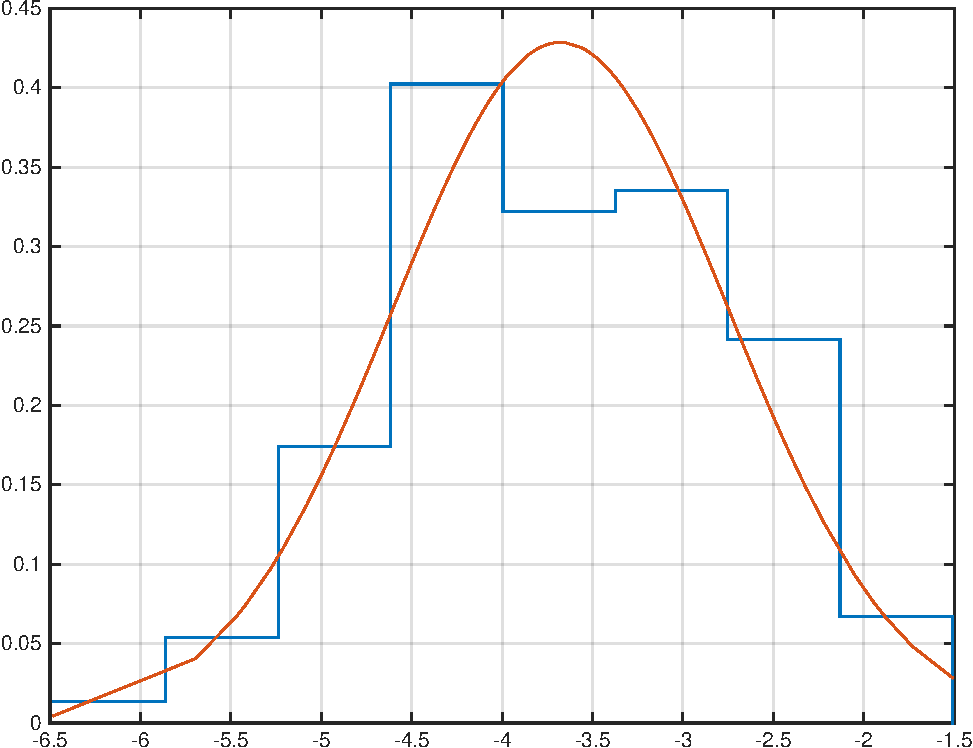
\includegraphics[width=0.7\textwidth]{graphic-1.pdf}
    \caption{График исходной выборки и полученной модели}
\end{figure}